\documentclass[aspectratio=169, 12pt]{beamer}

\usepackage[T2A]{fontenc}
\usepackage[utf8]{inputenc}
\usepackage[russian]{babel}
\usepackage{graphicx}
\usepackage{booktabs}
\usepackage{hyperref}
\usepackage{tikz}
\usepackage{xcolor}

\graphicspath{{img/}}

\usetheme{Madrid}
\usecolortheme{whale}

\setbeamertemplate{navigation symbols}{}
\setbeamertemplate{footline}{%
  \leavevmode%
  \hbox{%
    \begin{beamercolorbox}[wd=.333333\paperwidth,ht=2.25ex,dp=1ex,center]{author in head/foot}%
      \usebeamerfont{author in head/foot}\insertshortauthor
    \end{beamercolorbox}%
    \begin{beamercolorbox}[wd=.333333\paperwidth,ht=2.25ex,dp=1ex,center]{title in head/foot}%
      \usebeamerfont{title in head/foot}\insertshorttitle
    \end{beamercolorbox}%
    \begin{beamercolorbox}[wd=.333333\paperwidth,ht=2.25ex,dp=1ex,right]{date in head/foot}%
      \usebeamerfont{date in head/foot}\insertshortdate{}\hspace*{2em}
      \insertframenumber{} / \inserttotalframenumber\hspace*{2ex}
    \end{beamercolorbox}}%
  \vskip0pt%
}

\title[Молочная ферма]{Информационная система управления молочной фермой\\с интеграцией роботизированного оборудования\\и предиктивной аналитикой}
\author[ФИО студента]{ФИО СТУДЕНТА\\[0.5em]{\small Руководитель: ФИО РУКОВОДИТЕЛЯ}}
\institute{}
\date{2026}

\begin{document}

\begin{frame}
  \titlepage
\end{frame}

\begin{frame}{Содержание}
  \tableofcontents
\end{frame}

%% ============================================================
\section{Актуальность и постановка задачи}
%% ============================================================

\begin{frame}{Актуальность}
  \begin{itemize}
    \item Развитие концепции \textbf{точного животноводства} --- непрерывный автоматизированный мониторинг состояния животных
    \item Роботизированные доильные установки генерируют большие объёмы данных, требующих автоматизированной обработки
    \item Существующие решения --- закрытые, привязаны к одному производителю, не поддерживают собственные модели ML
    \item Необходима \textbf{открытая система}: полный цикл учёта + интеграция с оборудованием + предиктивная аналитика
  \end{itemize}
\end{frame}

\begin{frame}{Цель и задачи}
  \begin{block}{Цель}
    Разработка информационной системы управления молочной фермой с интеграцией оборудования Lely и предиктивной аналитикой на основе машинного обучения.
  \end{block}

  \vspace{0.8em}
  \textbf{Задачи:}
  \begin{enumerate}
    \item Спроектировать трёхзвенную архитектуру и модель данных (35+ таблиц)
    \item Реализовать серверный API на Rust/Axum (25+ модулей)
    \item Разработать веб-приложение на SvelteKit (24+ страницы)
    \item Реализовать модуль ML с 11 моделями
    \item Обеспечить интеграцию с Lely Horizon API (23 типа данных)
    \item Настроить мониторинг и CI/CD
  \end{enumerate}
\end{frame}

%% ============================================================
\section{Архитектура и технологии}
%% ============================================================

\begin{frame}{Стек технологий}
  \begin{columns}[T]
    \begin{column}{0.32\textwidth}
      \textbf{Backend}
      \begin{itemize}
        \item Rust + Axum
        \item SQLx + PostgreSQL
        \item TimescaleDB
        \item JWT + bcrypt
      \end{itemize}
    \end{column}
    \begin{column}{0.32\textwidth}
      \textbf{Frontend}
      \begin{itemize}
        \item SvelteKit 2
        \item Svelte 5 (Runes)
        \item Tailwind CSS 4
        \item Chart.js
      \end{itemize}
    \end{column}
    \begin{column}{0.32\textwidth}
      \textbf{Инфраструктура}
      \begin{itemize}
        \item Docker Compose
        \item Nginx + SSL
        \item Prometheus + Grafana
        \item GitHub Actions CI/CD
      \end{itemize}
    \end{column}
  \end{columns}
\end{frame}

\begin{frame}{Архитектура системы}
  \begin{center}
    
\includegraphics[width=0.85\textwidth,height=0.6\textheight,keepaspectratio]{container.png}
  \end{center}
  \begin{itemize}\small
    \item Nginx --- единая точка входа, терминация SSL, маршрутизация
    \item Backend --- бизнес-логика, интеграция с Lely, аналитика
    \item Analytics-ML --- 11 моделей машинного обучения (Python/FastAPI)
  \end{itemize}
\end{frame}

\begin{frame}{Модель данных}
  \begin{center}
    
\includegraphics[width=0.9\textwidth,height=0.7\textheight,keepaspectratio]{database-model.png}
  \end{center}
  \begin{itemize}\small
    \item 35+ таблиц PostgreSQL с TimescaleDB гипертаблицами
    \item 23 миграции, 10 доменных областей
  \end{itemize}
\end{frame}

%% ============================================================
\section{Серверная часть}
%% ============================================================

\begin{frame}{Backend: архитектура}
  \begin{center}
    
\includegraphics[width=0.85\textwidth,height=0.65\textheight,keepaspectratio]{backend-components.png}
  \end{center}
\end{frame}

\begin{frame}{Backend: безопасность}
  \begin{columns}[T]
    \begin{column}{0.48\textwidth}
      \textbf{Аутентификация}
      \begin{itemize}
        \item JWT (access + refresh), HS256
        \item HttpOnly, SameSite=Strict cookies
        \item Token revocation через БД
        \item Роли: admin / user
      \end{itemize}
    \end{column}
    \begin{column}{0.48\textwidth}
      \textbf{Защита}
      \begin{itemize}
        \item Rate limiting (Redis / in-memory)
        \item CSRF-защита (Origin header)
        \item AES-256-GCM (учётные данные Lely)
        \item Prometheus metrics
      \end{itemize}
    \end{column}
  \end{columns}
\end{frame}

%% ============================================================
\section{Клиентское приложение}
%% ============================================================

\begin{frame}{Frontend: архитектура}
  \begin{center}
    
\includegraphics[width=0.85\textwidth,height=0.65\textheight,keepaspectratio]{frontend-structure.png}
  \end{center}
  \begin{itemize}\small
    \item 20+ маршрутов, 20 API-модулей, 22 компонента, 19 утилит
    \item SSR + PWA, Chart.js визуализация, Tailwind CSS 4
  \end{itemize}
\end{frame}

%% ============================================================
\section{Машинное обучение}
%% ============================================================

\begin{frame}{Модели машинного обучения}
  \begin{center}
    \begin{tabular}{lll}
      \toprule
      \textbf{Модель} & \textbf{Алгоритм} & \textbf{Назначение} \\
      \midrule
      Прогноз надоев (корова) & XGBoost & Дневной надой + q10/q90 \\
      Прогноз надоев (стадо) & Prophet & Тренд + сезонность \\
      Риск мастита & XGBoost & Классификация риска \\
      Предупреждение кетоза & XGBoost & Классификация риска \\
      Обнаружение охоты & XGBoost & Классификация состояния \\
      Риск выбраковки & XGBoost & Дни до выбраковки \\
      Кластеризация стада & KMeans & Сегментация \\
      Аномалии оборудования & Isolation Forest & Детекция аномалий \\
      \bottomrule
    \end{tabular}
  \end{center}
  \vspace{0.5em}
  \textbf{MLOps:} автообучение, Optuna оптимизация, мониторинг дрейфа, SHAP объяснимость, MLflow логирование
\end{frame}

\begin{frame}{Аналитические алгоритмы (Rust)}
  \begin{itemize}
    \item \textbf{Хольт--Винтерс} --- тройное экспоненциальное сглаживание для прогнозирования надоев с учётом уровня, тренда и сезонности (7 дней)
    \item \textbf{Кривая Вуда} --- лог-линейная модель $y(t) = a \cdot t^b \cdot e^{-ct}$ лактации, определение пика $t_{\max} = -b/c$
    \item \textbf{Индекс здоровья} --- составной показатель на основе z-оценок надоев, SCC, активности и жвачки
    \item \textbf{Оптимизатор запуска} --- расчёт даты сухостойного периода с учётом текущего надоя
  \end{itemize}
\end{frame}

%% ============================================================
\section{Интеграция с Lely}
%% ============================================================

\begin{frame}{Интеграция с Lely Horizon}
  \begin{itemize}
    \item Автоматическая синхронизация каждые 5 минут по настраиваемому таймеру
    \item \textbf{23 типа данных}: животные, отёлы, осеменения, надои, качество молока, кормление, активность, жвачка, данные роботов
    \item Инкрементальная синхронизация по временным диапазонам (чанками по 7 дней)
    \item Шифрование учётных данных AES-256-GCM
    \item Автообновление токена каждые 58 минут, retry с экспоненциальной задержкой
    \item Конфигурация через веб-интерфейс без перезапуска сервера
  \end{itemize}
\end{frame}

%% ============================================================
\section{Мониторинг и развёртывание}
%% ============================================================

\begin{frame}{Мониторинг (Grafana LGTM)}
  \begin{center}
    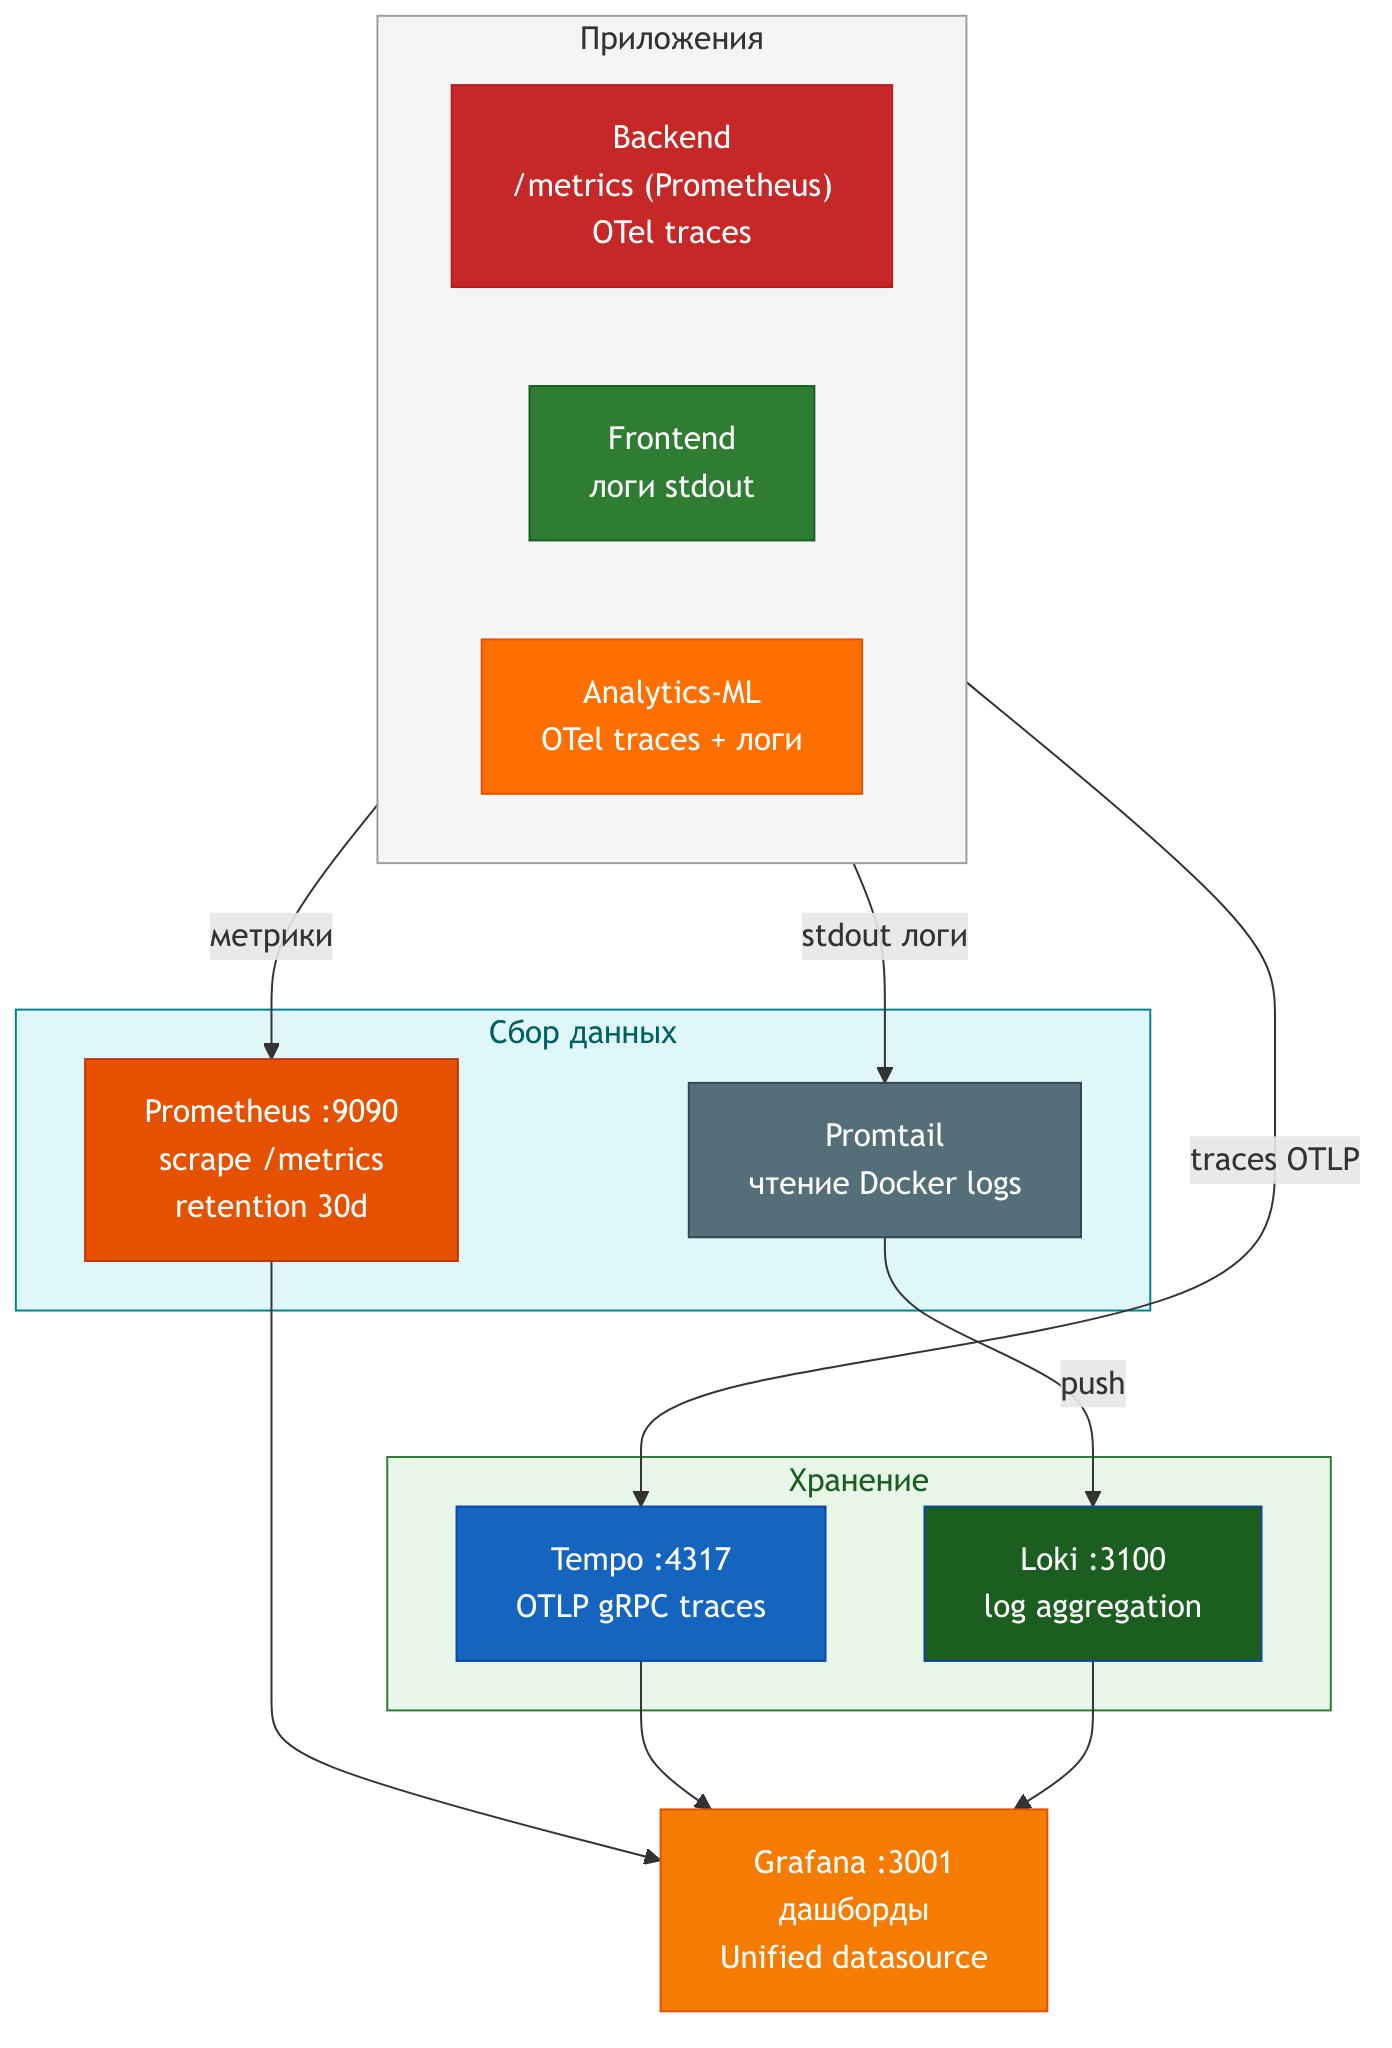
\includegraphics[width=0.85\textwidth,height=0.6\textheight,keepaspectratio]{monitoring.png}
  \end{center}
  \begin{itemize}\small
    \item Prometheus --- метрики backend, ML, Redis (30d retention)
    \item Grafana --- дашборды с преднастроенными панелями
    \item Loki + Promtail --- агрегация логов из Docker-контейнеров
    \item Tempo --- распределённая трассировка через OTLP
  \end{itemize}
\end{frame}

\begin{frame}{CI/CD и развёртывание}
  \begin{columns}[T]
    \begin{column}{0.48\textwidth}
      \textbf{CI/CD (GitHub Actions)}
      \begin{center}
        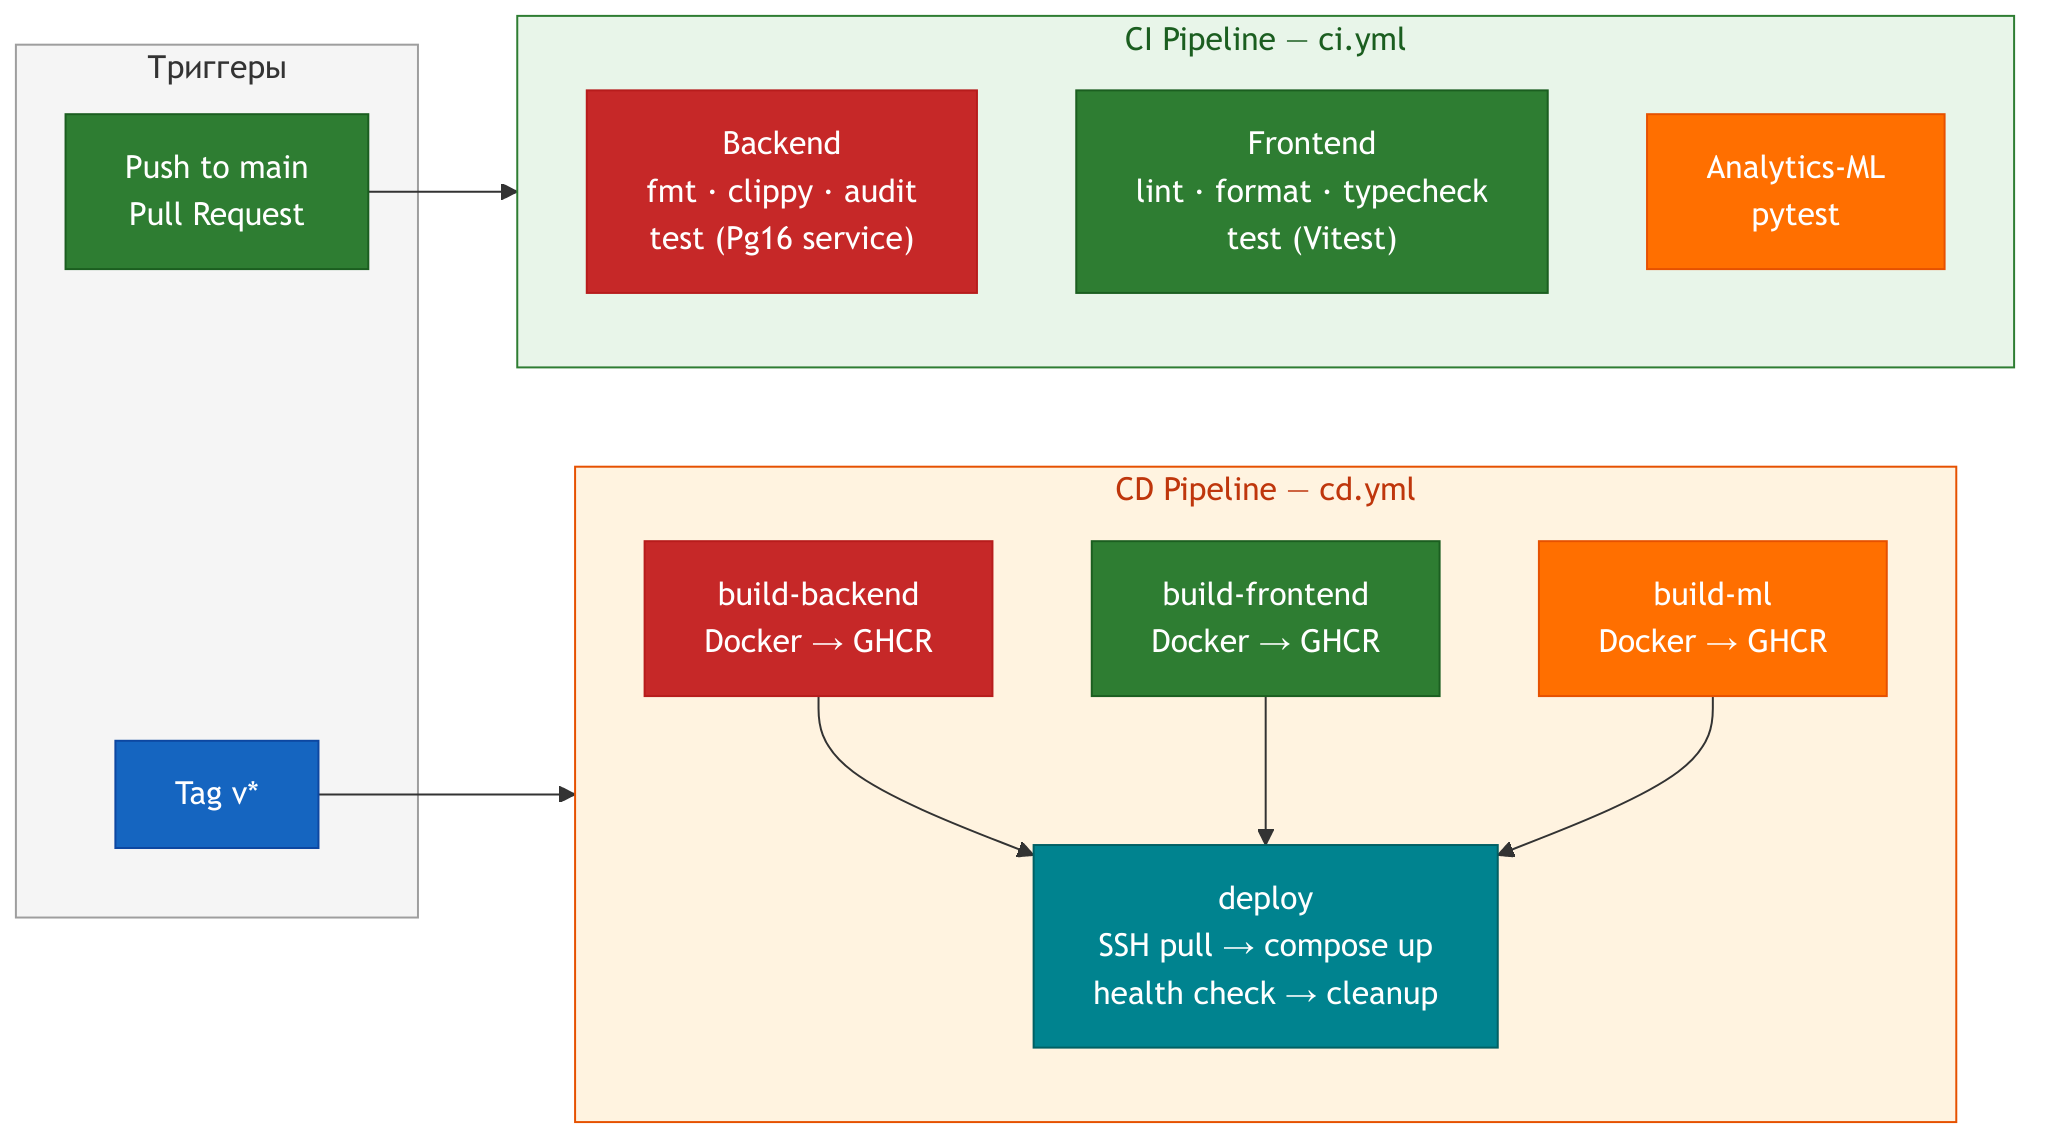
\includegraphics[width=\textwidth,height=0.55\textheight,keepaspectratio]{ci-cd.png}
      \end{center}
    \end{column}
    \begin{column}{0.48\textwidth}
      \textbf{Развёртывание (Docker Compose)}
      \begin{center}
        
\includegraphics[width=\textwidth,height=0.55\textheight,keepaspectratio]{deployment.png}
      \end{center}
    \end{column}
  \end{columns}
  \vspace{0.3em}
  \begin{itemize}\small
    \item CI: fmt, clippy, audit, test (3 параллельных потока)
    \item CD: Docker build $\to$ GHCR $\to$ SSH deploy + health check
    \item Prod: SSL, rate limiting, resource limits, log rotation
  \end{itemize}
\end{frame}

%% ============================================================
\section{Результаты}
%% ============================================================

\begin{frame}{Результаты}
  \begin{columns}[T]
    \begin{column}{0.48\textwidth}
      \textbf{Количественные показатели}
      \begin{itemize}
        \item 25+ модулей обработчиков API
        \item 33 модуля бизнес-логики
        \item 35+ таблиц базы данных
        \item 24+ страниц frontend
        \item 11 моделей машинного обучения
        \item 17+ типов отчётов (CSV/PDF)
        \item 30+ файлов тестов
      \end{itemize}
    \end{column}
    \begin{column}{0.48\textwidth}
      \textbf{Качественные показатели}
      \begin{itemize}
        \item Rust --- безопасность памяти и производительность
        \item SvelteKit --- быстрый и отзывчивый UI
        \item XGBoost --- раннее обнаружение заболеваний
        \item Docker --- готовность к продакшену
        \item Grafana LGTM --- полное наблюдение
        \item CI/CD --- автоматический деплой
      \end{itemize}
    \end{column}
  \end{columns}
\end{frame}

%% ============================================================
\section{Заключение}
%% ============================================================

\begin{frame}{Заключение}
  \begin{itemize}
    \item Разработана информационная система управления молочной фермой с полным циклом: от учёта до предиктивной аналитики
    \item Реализована интеграция с роботизированным оборудованием Lely (23 типа данных, шифрование)
    \item Модуль ML из 11 моделей: прогноз надоев, мастит, кетоз, охота, выбраковка, кластеризация, аномалии оборудования
    \item Система развёрнута в Docker с мониторингом, SSL и CI/CD
    \item \textbf{Дальнейшее развитие:} интеграция с другими производителями, мобильное приложение, финансовый анализ
  \end{itemize}
\end{frame}

\begin{frame}{}
  \begin{center}
    \Huge Спасибо за внимание!
  \end{center}
\end{frame}

\end{document}
